\documentclass{scrartcl}

\usepackage{german}
\usepackage[utf8]{inputenc}  %Umlaute
\usepackage[T1]{fontenc}     %Umlauttrennung
\usepackage{lmodern}         %modernes Schriftbild
\usepackage{amsmath}         %math Umgebungen
\usepackage{graphicx}
\usepackage{hyperref}        %URLs
\usepackage{gensymb}         %Gradzeichen
\usepackage{float}           %Positionierung von Tabellen und Abb

\title{Physikpraktikum für Naturwissenschaftler \\ Versuch: Oberflächenspannung}
\author{Felix Burr, Johannes Spindler (Gruppe 13)}
\date{Durchgeführt am 08. November 2018}


\begin{document}
\begin{titlepage}
  \begin{center}
    \vspace*{1cm}
    \LARGE
    Physikpraktikum für Naturwissenschaftler \\
    \vspace*{1cm}
    \Huge
    \textbf{Versuch: Oberflächenspannung} \\
    \vspace*{0.3cm}
    \Large
    Durchgeführt am 08. November 2018 \\
    Betreuerin: Sabrina Hartmann \\
    \vspace*{2.5cm}
    Gruppe 13 \\
    Felix Burr: felix.burr@uni-ulm.de \\
    Johannes Spindler: johannes.spindler@uni-ulm.de \\
    \vfill 
  \end{center}
  Wir bestätigen hiermit, das Protokoll selbstständig erarbeitet zu haben und in genauer Kenntnis über dessen Inhalt zu sein. \\
  \vspace*{0.8cm}
  \\
  Felix Burr
  \hfill
  Johannes Spindler
\end{titlepage}
\pagebreak
\tableofcontents


\pagebreak

\section{Einleitung}
Wer einen Wassertropfen am Ende einer Wasserhahns hängen sieht, bemerkt, dass sich dieser wie eine gedehnte Membran unter Spannung verhält und sich zu einer Kugel formt. Diese Spannung entsteht durch ionische Coulombkräfte, Dipol-Dipol-Kräfte und Van-der-Waals-Kräfte zwischen den Molekülen in Flüssigkeiten und wird als Oberflächenspannung bezeichnet.

Im Folgenden werden verschiedene Methoden zur Bestimmung der Oberflächenspannung verschiedener Flüssigkeiten angewandt und deren Ergebnisse diskutiert.
\section{Oberflächenspannung von Wasser, Ethanol und Kochsalzlösung (Abreißmethode)}
\subsection{Versuchsdurchführung}

Der Versuchsaufbau besteht aus einem Behältnis mit Flüssigkeit, das auf einem Podest mit verstellbarer Höhe steht. An einer Federwaage über diesem hängt ein Ring mit scharfer Schneide. Dessen Radius $r$ wird mit einer Schieblehre bestimmt. Das Podest wird zu Beginn so eingestellt, dass der Ring in der Flüssigkeit hängt, dann wird es heruntergefahren. Dabei bildet sich eine Flüssigkeitslamelle am Rand des Rings. Die Skala der Federwaage muss dabei im Auge behalten werden. Schließlich wird die Kraft $F$ in dem Moment abgelesen, indem die Lamelle abreißt, was diesem Vorgehen den Namen Abreißmethode gibt.

\begin{figure}[H]
  \centering
    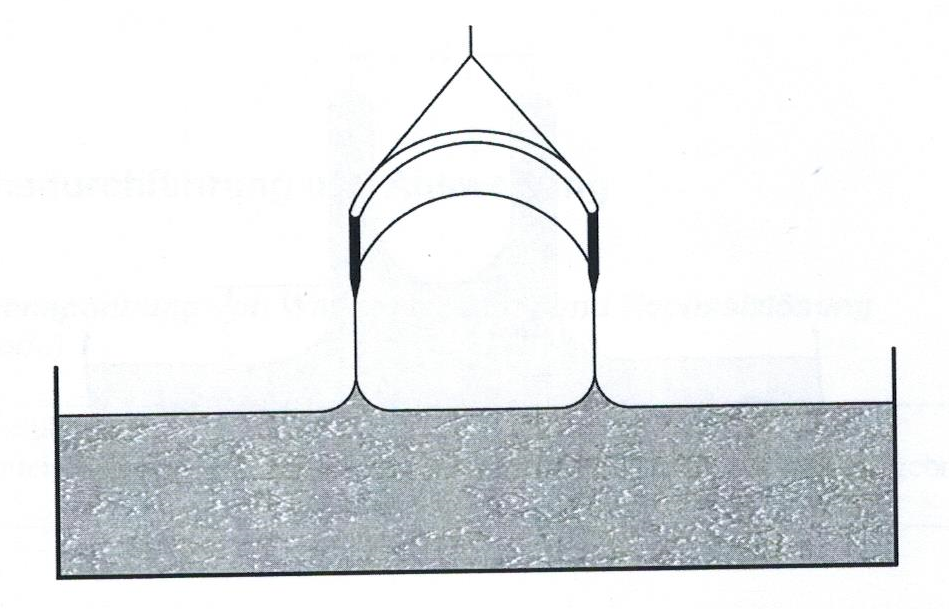
\includegraphics[scale=0.75]{Abreiss.PNG}
  \caption{Der Versuchsaufbau zur Abreißmethode (aus der Versuchsanleitung)}
  \label{fig:Abreiss}
\end{figure}

Die Oberflächenspannung $\sigma$ ist allgemein definiert als
\begin{align}
\sigma = \dfrac{\Delta W}{\Delta O}
\label{eq:sigma1}
\end{align}
wobei $\Delta O$ eine hinzugewonnene Flüssigkeitsoberfläche und $\Delta W$ die dafür benötigte Energie ist.
Beim Ansteigen der Lamelle um die Höhendifferenz $\Delta h$ muss entgegen der abgelesenen Kraft $F$ gearbeitet werden, welche die Resultierende aus oben erwähnten zwischenmolekularen Kräften und der Gewichtskraft ist.
\begin{align}
\Delta W = F \cdot \Delta h
\end{align}
Es bildet sich eine röhrenförmige Lamelle mit vernachlässigbarer Dicke. Sei $A$ die Außenfläche dieser Lamelle (die Innenfläche ist wegen geringer Dicke auch $A$), dann ist die zugewonnene Oberfläche $\Delta O$ gegeben durch
\begin{align}
\Delta O = 2A = 2(2 \pi r \cdot \Delta h) = 4 \pi r \cdot \Delta h
\label{eq:delta_O}
\end{align}
In Gleichung \ref{eq:sigma1} eingesetzt ergibt das für die Oberflächenspannung
\begin{align}
\sigma = \dfrac{F \cdot \Delta h}{4 \pi r \cdot \Delta h} = \dfrac{F}{4 \pi r} \label{eq:sigma2}
\end{align}
\subsection{Messwerte und Ergebnisse}
Ringdurchmesser 6,5cm, also $r = 0,0325m$

Raumtemperatur: $21,9 \degree C$
\subsubsection{Messungen bei Wasser}

\begin{table}[H]
\captionof{table}{Kraft $F$ und Oberflächenspannung $\sigma$ bei Wasser}
\begin{center}
\begin{tabular}{l|l|l}
Messung    & $F$ {[}mN{]} & $\sigma$ {[}N/m{]} \\
\hline
1          & 24,0       & 0,0588    \\
2          & 24,0       & 0,0588    \\
3          & 25,5       & 0,0624    \\
Mittelwert & 24,5       & 0,0600                    
\end{tabular}
\end{center}
\label{tab:Wasser}
\end{table}
\subsubsection{Messungen bei Ethanol}

\begin{table}[H]
\captionof{table}{Kraft $F$ und Oberflächenspannung $\sigma$ bei Ethanol}
\begin{center}
\begin{tabular}{l|l|l}
Messung    & $F$ {[}mN{]} & $\sigma$ {[}N/m{]} \\
\hline
1          & 7,0       & 0,0171    \\
2          & 7,0       & 0,0171    \\
3          & 7,0       & 0,0171    \\
Mittelwert & 7,0       & 0,0171                    
\end{tabular}
\end{center}
\label{tab:Ethanol}
\end{table}
\subsubsection{Messungen bei Kochsalzlösung}

\begin{table}[H]
\captionof{table}{Kraft $F$ und Oberflächenspannung $\sigma$ bei Kochsalzlösung}
\begin{center}
\begin{tabular}{l|l|l}
Messung    & $F$ {[}mN{]} & $\sigma$ {[}N/m{]} \\
\hline
1          & 22,0       & 0,0539    \\
2          & 20,0       & 0,0490    \\
3          & 19,0       & 0,0465    \\
Mittelwert & 20,3       & 0,0498                    
\end{tabular}
\end{center}
\label{tab:Kochsalz}
\end{table}
\subsection{Fehlerrechnung}
Aus Gleichung \ref{eq:sigma2} folgt für $\sigma$, das von den Messgrößen $F$ und $r$ abhängt, der Größtfehler
\begin{align*}
\Delta \sigma = \left| \dfrac{\partial \sigma}{\partial F} \right| \Delta F + \left| \dfrac{\partial \sigma}{\partial r} \right| \Delta r = \left| \dfrac{1}{4 \pi r} \right| \Delta F + \dfrac{F}{4 \pi} \left| - \dfrac{1}{r^2} \right| \Delta r =\dfrac{1}{4 \pi r} \Delta F + \dfrac{F}{4 \pi r^2} \Delta r
\end{align*}
Da die Skala auf dem Kraftmesser in Abständen von einem Milli-Newton aufgetragen ist und zum Messen des Ringradius eine Schieblehre verwendet wurde, werden $\Delta F = 1mN, \Delta r = 0,05mm$ als Größtfehler angenommen.

\subsubsection{Standardabweichung und Größtfehler von $\sigma$ bei Wasser}
Aus Tabelle \ref{tab:Wasser} folgt eine Standardabweichung von 0,0021. Mit den Mittelwerten $F = 24,5mN, \sigma = 0,0600N/m$ ergibt sich der Größtfehler von $\sigma$:
\begin{align*}
\Delta \sigma & = \dfrac{1}{4 \pi \cdot 0,0325m} 0,0010N + \dfrac{0,0245N}{4 \pi (0,0325m)^2} 5 \cdot 10^{-5}m = 0,00254N \\
\sigma & = 0,0600N \pm 0,00254N
\end{align*}
\subsubsection{Standardabweichung und Größtfehler von $\sigma$ bei Ethanol}
Wie in Tabelle \ref{tab:Ethanol} zu sehen ist, wurde in allen drei Messungen derselbe Wert für die Kraft gemessen, weshalb die Standardabweichung Null beträgt. Mit den Mittelwerten $F = 7,0mN, \sigma = 0,0171N/m$ ergibt sich der Größtfehler von $\sigma$:
\begin{align*}
\Delta \sigma & = \dfrac{1}{4 \pi \cdot 0,0325m} 0,0010N + \dfrac{0,0070N}{4 \pi (0,0325m)^2} 5 \cdot 10^{-5}m = 0,00247N \\
\sigma & = 0,0171N \pm 0,00247N
\end{align*}
\subsubsection{Standardabweichung und Größtfehler von $\sigma$ bei Kochsalzlösung}
Aus Tabelle \ref{tab:Kochsalz} folgt eine Standardabweichung von 0,0037. Mit den Mittelwerten $F = 20,3mN, \sigma = 0,0498N/m$ ergibt sich der Größtfehler von $\sigma$:
\begin{align*}
\Delta \sigma & = \dfrac{1}{4 \pi \cdot 0,0325m} 0,0010N + \dfrac{0,0203N}{4 \pi (0,0325m)^2} 5 \cdot 10^{-5}m = 0,00253N \\
\sigma & = 0,0498N \pm 0,00253N
\end{align*}
\subsection{Ergebnisdiskussion}
Da die Raumtemperatur $22,9 \degree C$ betrug, werden zum Vergleich die Literaturwerte für die Oberflächenspannung bei $25 \degree C$ aus der Versuchsanleitung herangezogen, die Temperaturabweichung wird vernachlässigt.

Das Messergebnis $\sigma_{Wasser} = 0,0600N/m$ unterschreitet den Literaturwert von \\$0,07199N/m$ um 16,7\%.

Das Messergebnis $\sigma_{Ethanol} = 0,0171N/m$ unterschreitet den Literaturwert von \\$0,02197N/m$ um 22,2\%.

Das Messergebnis $\sigma_{NaCl-Lsg} = 0,0498N/m$ unterschreitet den Literaturwert von \\$0,082N/m$ um 39,3\%.

Da alle drei Messergebnisse unter den Literaturwerten liegen, müssen entweder die Werte für $F$ zu niedrig oder $\Delta O$ mit Gleichung \ref{eq:delta_O} überschätzt worden sein. Die Form der Lamelle wurde als zylindrisch angenommen, aber da der Ring nicht perfekt kreisförmig ist und die Wasseroberfläche mit der Lamelle nicht einen rechten Winkel bildet, ist der Zylinder nur eine Annäherung. Außerdem wurde die Dicke der Lamelle vernachlässigt, damit Außen- und Innenfläche als gleich groß angenommen werden können.
Beim Messen der Kraft ist das Problem, genau zum Zeitpunkt des Abreißens abzulesen.
Außerdem bleiben trotz Säubern des Behälters Verunreinigungen der Flüssigkeiten zurück und bei der Kochsalzlösung kann nicht gewährleistet werden, dass sie genau 3-molar vorbereitet wurde.
\newpage
\section{Oberflächenspannung von Tensidlösungen}
\subsection{Versuchsdurchführung}
Der Versuchsaufbau ist derselbe wie im vorherigen Versuchsteil. Diesmal wird als Flüssigkeit eine SDS-Lösung verwendet. Dazu werden 250ml einer 50 mM SDS-Stammlösung angesetzt.
Bei der ersten Messung wird die Oberflächenspannung von 500ml Wasser bestimmt, dann wird bei jeder nachfolgenden Messung eine vorgegebene Menge SDS-Stammlösung hinzugefügt und homogen vermischt.
In 13 Messungen werden damit SDS-Konzentration und Oberflächenspannung abhängig von der zugegebenen SDS-Menge (zwischen 0ml und 220ml) bestimmt.

Die SDS-Konzentration $C_{F}$ der Flüssigkeit kann abhängig vom Volumen $V_{F}$ der Flüssigkeit, dem Volumen $V_{SDS}$ der Stammlösung und der Konzentration $C_{SDS}$ der Stammlösung bestimmt werden durch
\begin{align}
C_{F} = \dfrac{C_{SDS} \cdot V_{SDS}}{V_{F}} = \dfrac{0,05 \dfrac{mol}{l} \cdot V_{SDS}}{0,5l + V_{SDS}}
\end{align}
Die Oberflächenspannung kann wieder mit Gleichung \ref{eq:sigma2} bestimmt werden.

Übersteigt $C_{F}$ die kritische Micellenkonzentration $CMC$, kann haben keine weiteren SDS-Moleküle mehr Platz an der Wasseroberfläche und die Oberflächenspannung bleibt konstant. Die $CMC$ soll durch die Messungen abgeschätzt werden.
\subsection{Messwerte und Ergebnisse}
\begin{table}[H]
\captionof{table}{SDS-Konzentration $C_{F}$ der Flüssigkeit, Kraft $F$ und Oberflächenspannung $\sigma$ abhängig von zugegebenem SDS-Volumen $V_{SDS}$}
\begin{center}
\begin{tabular}{l|l|l|l|l}
Messung & $V_{SDS}$ [ml]    & $C_{F}$ [mol/l]          & $F$ [mN]     & $\sigma$ [N/m]       \\
\hline
1       & 0   & 0,0000000 & 27,0 & 0,0661 \\
2       & 1   & 0,0000998 & 26,5 & 0,0649 \\
3       & 2   & 0,0001992 & 24,5 & 0,0600 \\
4       & 5   & 0,0004951 & 18,0 & 0,0441 \\
5       & 10  & 0,0009804 & 13,5 & 0,0331 \\
6       & 20  & 0,0019231 & 15,5 & 0,0380 \\
7       & 40  & 0,0037037 & 12,0 & 0,0294 \\
8       & 60  & 0,0053571 & 11,0 & 0,0269 \\
9       & 80  & 0,0068966 & 10,5 & 0,0257 \\
10      & 100 & 0,0083333 & 10,0 & 0,0245 \\
11      & 120 & 0,0096774 & 11,0 & 0,0269 \\
12      & 170 & 0,0126866 & 11,5 & 0,0282 \\
13      & 220 & 0,0152778 & 12,0 & 0,0294
\end{tabular}
\end{center}
\label{tab:SDS}
\end{table}
\subsection{Ergebnisdiskussion}

\begin{figure}[H]
  \centering
    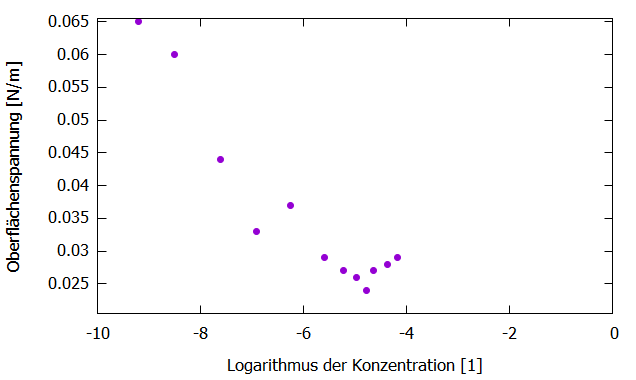
\includegraphics[scale=0.90]{plot_sigma.PNG}
  \caption{Zusammenhang zwischen $ln(C_{F})$ und $\sigma$ aus Tabelle \ref{tab:SDS}}
  \label{fig:plot_sigma}
\end{figure}

Wie in Abbildung \ref{fig:plot_sigma} zu sehen ist, konzentrieren sich die $\sigma$-Werte der Messungen 11 bis 13 um etwa $0,028N/m$, während $\sigma$ zwischen den Messungen 1 bis 11 (mit Ausnahme von Messung 6) von $0,066N/m$ auf $0,024N/m$ monoton (vermutlich linear) fällt.

Es ist also anzunehmen, dass die kritische Micellkonzentration $CMC$ etwa bei Messung 11 liegt, was dann $CMC \approx 0,0083 mol/l$ entspricht. Der Vergleich mit dem Literaturwert von $0,0081 mol/l$ ergibt eine Abweichung von 2,5\%.

Ungenauigkeiten treten wie im vorherigen Versuch erklärt wegen der Näherung der Oberfläche als Zylinder, wegen Verunreinigungen und Ablesen der Kraft zum falschen Zeitpunkt auf.
Zusätzlich kommt hinzu, dass die Zugabe von Stammlösung durch eine Pipette nicht genau ist und das SDS eventuell nicht immer homogen mit dem Wasser vermischt war, wodurch sich eine SDS-Phase auf dem Wasser bildet.
\newpage 
\section{Oberflächenspannung von Wasser und einer SDS-Lösung (Kapillarmethode)}
\subsection{Versuchsdurchführung}
\begin{figure}[H]
  \centering
    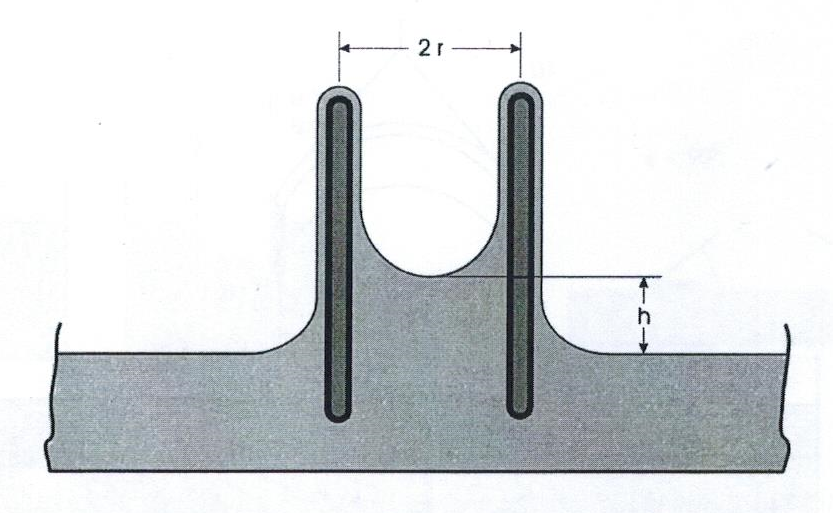
\includegraphics[scale=0.75]{Kapillar.PNG}
  \caption{Der Versuchsaufbau zur Kapillarmethode (aus der Versuchsanleitung)}
  \label{fig:Kapillar}
\end{figure}
\subsection{Messwerte und Ergebnisse}
\begin{table}[H]
\captionof{table}{Steighöhe von Wasser in Abhängigkeit des Kapillardurchmessers}
\begin{center}
\begin{tabular}{l|l|l|l|l}
Röhre & Kapillardurchmesser $[m]$& Wasseroberfläche $[m]$ & Meniskus $[m]$ & Steighöhe $[m]$       \\
\hline
1       & 0,005   	& 0,01 & 0,013 		& 0,003 \\
2       & 0,0031   	& 0,01 & 0,0184 	& 0,0084 \\
3       & 0,00165   & 0,01 & 0,0277		& 0,0177 \\
4       & 0,0012   	& 0,01 & 0,0349		& 0,0249 \\
5       & 0,00083	& 0,01 & 0,0465		& 0,0365 \\
\end{tabular}
\end{center}
\label{tab:Steig_W}
\end{table}

\begin{table}[H]
\captionof{table}{Steighöhe von SDS in Abhängigkeit des Kapillardurchmessers}
\begin{center}
\begin{tabular}{l|l|l|l}
Röhre & Kapillardurchmesser $[m]$& Steighöhe $[pixel]$ & Steighöhe $[m]$       \\
\hline
1       & 0,005   	& 20 	& 0,0038 \\
2       & 0,0031   	& 27 	& 0,0052 \\
3       & 0,00165   & 70	& 0,0136 \\
4       & 0,0012   	& 73	& 0,0142 \\
5       & 0,00083	& 180	& 0,0349 \\
\end{tabular}
\end{center}
\label{tab:Steig_S}
\end{table}
\subsection{Ergebnisdiskussion}
\begin{figure}[H]
  \centering
    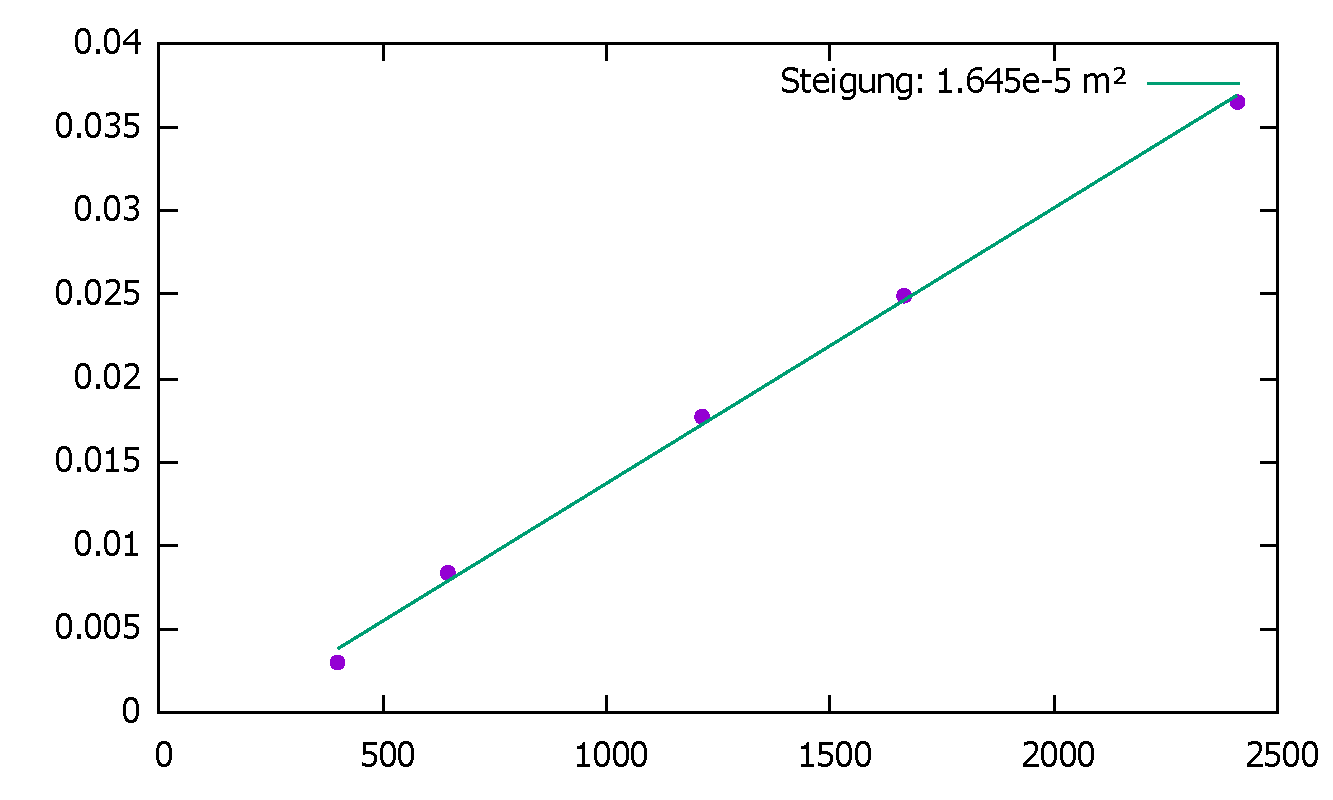
\includegraphics[scale=0.6]{pypr_OV3W.pdf}
  \caption{Lineare Regression über Tabelle 5}
  \label{fig:Steig_W}
\end{figure}
\begin{figure}[H]
  \centering
    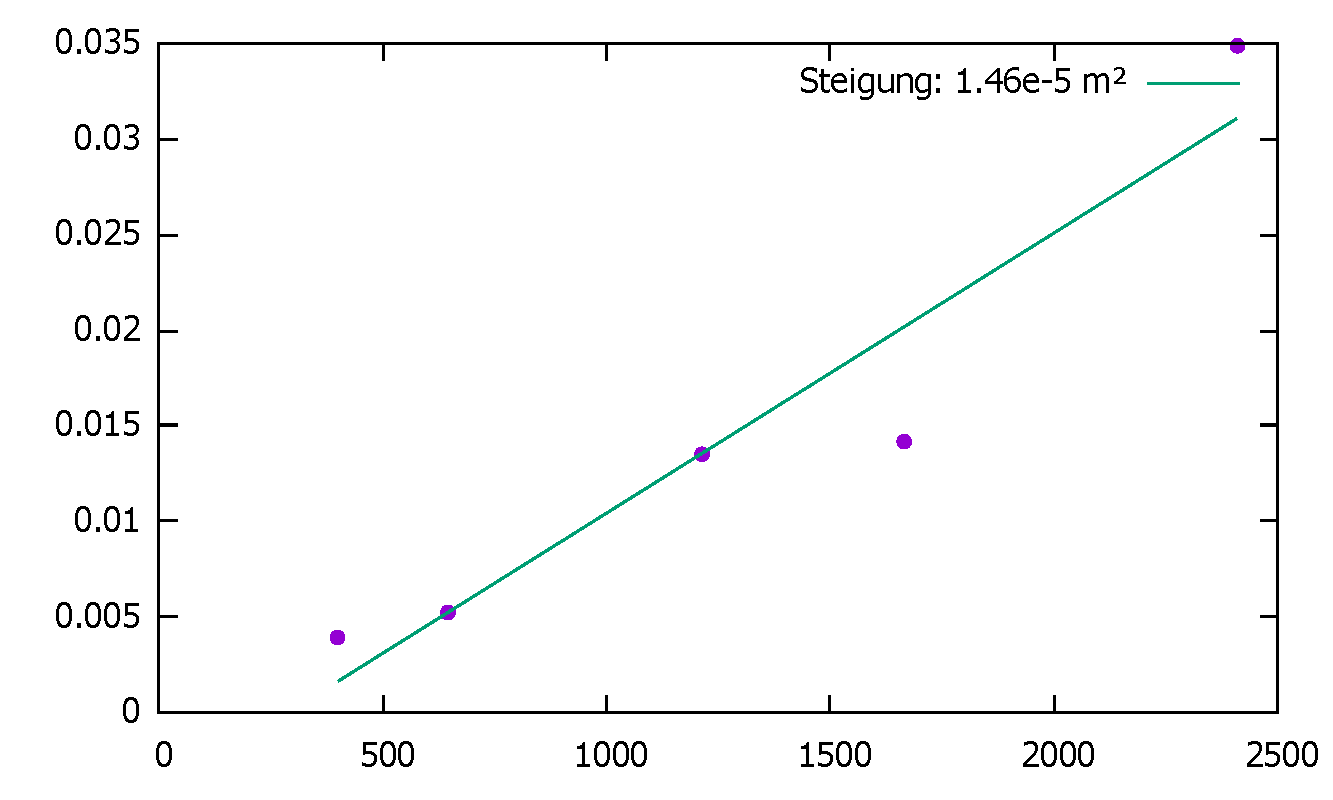
\includegraphics[scale=0.6]{pypr_OV3S.pdf}
  \caption{Lineare Regression über Tabelle 6}
  \label{fig:Steig_S}
\end{figure}
Wie in Abbildung \ref{tab:Steig_W} und \ref{tab:Steig_S} zu sehen ist, verhält sich das Inverse des Kapillardurchmessers linear zur Steighöhe. Durch die Steigung der Geraden können wir mittels
\begin{align}
\sigma = \dfrac{1}{2}\cdot \rho \cdot g \cdot h \cdot r 
\label{eq:sigma_V3}
\end{align}
Die Oberflächenspannung bestimmen.
Bei Wasser haben wir eine Oberflächenspannung von $\sigma = 73,35 \frac{mN}{m}$ ermittelt. Im Vergleich zum Literaturwert von $72.5 \frac{mN}{m}$ weicht der gemessene Wert um $1.16\%$ ab, was vor allem auf den Temperaturunterschied oder potentielle Verschmutzungen des Wassers und des Kapillars zurückzuführen ist.
Bei SDS haben wir hingegen eine Oberflächenspannung von $\sigma = 71,40 \frac{mN}{m}$ ermittelt. Im vorhergehenden Versuch erhielten wir dafür einen Wert von $\sigma = 29,4 \frac{mN}{m}$. Was überhaupt nicht mit dem aktuellen Wert übereinstimmt.
Eine Erklärung dafür wäre die Möglichkeit, dass die SDS Lösung mit Wasser vertauscht bzw. verwechselt wurde.

\newpage
\section{Benetzung von Oberflächen}
\subsection{Versuchsdurchführung}
In diesem Versuch untersuchen wir die Vernetzung von Oberflächen, indem wir mit einer Pipette einen Wassertropfen auf eine Glasplatte fallen lassen,  die einmal kalt (Raumtemperatur) und einmal heiß (erhitzen via Bunsenbrenner) ist.
Wir beobachten nun, wie sich der Wassertropfen auf der Oberfläche jeweils verhält. 

\subsection{Ergebnisdiskussion}


\end{document}
